\documentclass[12pt]{article}

%----------------------------
% PACKAGES
%----------------------------
\usepackage[utf8]{inputenc}
\usepackage{amsmath, amssymb}
\usepackage{graphicx}
\usepackage{hyperref}
\usepackage{geometry}
\usepackage{caption}
\usepackage{fancyhdr}
\usepackage{xcolor}
\usepackage{listings}
\usepackage{enumitem}
\usepackage{titlesec}
\usepackage{hyperref}
\usepackage{url}
\usepackage{float}

%----------------------------
% PAGE GEOMETRY & HEADER
%----------------------------
\geometry{margin=1in}
\pagestyle{fancy}
\fancyhf{}
\rhead{Redshift Estimation}
\lhead{Ripley Sinclair}
\cfoot{\thepage}

%----------------------------
% CODE STYLE
%----------------------------
\lstset{
  basicstyle=\ttfamily\footnotesize,
  backgroundcolor=\color{gray!10},
  frame=single,
  breaklines=true
}

%----------------------------
% TITLE FORMAT
%----------------------------
\titleformat{\section}
  {\normalfont\Large\bfseries}{\thesection}{1em}{}
\titleformat{\subsection}
  {\normalfont\large\bfseries}{\thesubsection}{1em}{}

%----------------------------
% DOCUMENT
%----------------------------
\begin{document}

%----------------------------
% TITLE PAGE
%----------------------------
\begin{titlepage}
    \centering
    {\scshape\LARGE Mapping The Cosmos Through Redshift Estimation \par}
    \vspace{1.5cm}
    {\Large\itshape Ripley Sinclair\par}
    \vfill
    {\large \today\par}
\end{titlepage}

%----------------------------
% ABSTRACT
%----------------------------

\section{Introduction}

This work explores how astronomers estimate redshift, the measure of how light from distant galaxies is stretched by the expansion of the universe. The process began with synthetic spectra to understand how spectral lines shift in wavelength and progressed toward processing real observational data using tools such as cross-correlation and template matching. Common pitfalls encountered include poor normalization, noisy signals, and unrealistic templates.

\section{Simulated Spectra and Initial Methods}

To build foundational understanding, synthetic spectra were generated composed of Gaussian emission lines located at known rest-frame wavelengths. These simplified datasets allowed for clean experimentation without real-world noise or instrumental artifacts.


\paragraph{Initial Feature Detection}
The first technique involved direct peak detection using a custom implementation of \texttt{find\_peaks}. This method performed well on clean synthetic spectra, as sharp emission lines stood out clearly from the baseline. However, when noise or baseline shifts were introduced, this method became unreliable.

\begin{figure}[H]
    \centering
    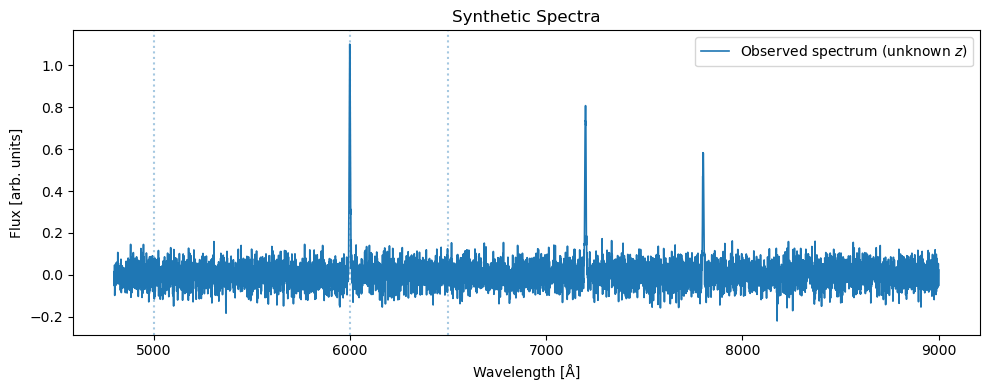
\includegraphics[width=1\linewidth]{image.png}
    \caption{Synthetic Spectra}
    \label{fig:placeholder}
\end{figure}

\begin{figure}[H]
    \centering
    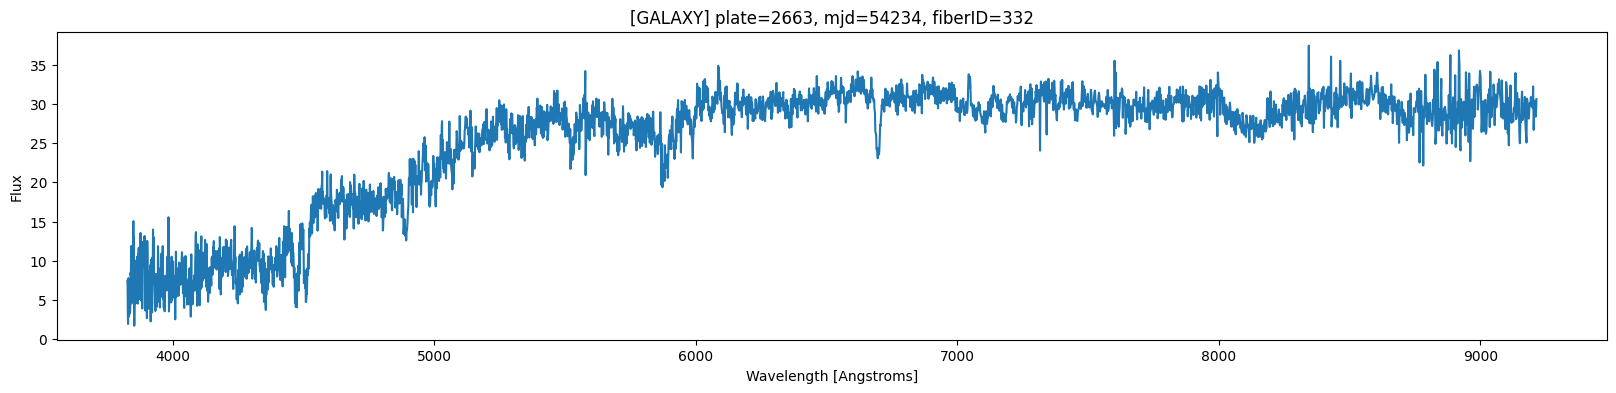
\includegraphics[width=1\linewidth]{image2.png}
    \caption{Real Spectra [GALAXY] plate=2663, mjd=54234, fiberID=332}
    \label{fig:real}
\end{figure}


\section{Cross-Correlation and Template Matching}

After limitations in direct peak detection became evident, a cross-correlation pipeline was implemented using Gaussian-based templates. Each template consisted of Gaussian features positioned at rest-frame wavelengths corresponding to known emission lines (e.g., Ly-$\alpha$, CIV, OIII).

To compute redshift, the following steps were applied:
\begin{itemize}
\item Construction of a logarithmic redshift grid \cite{baldry2018logredshift}.
\item Resampling of both template and observed spectra in log-wavelength space \cite{baldry2018logredshift}.
\item Normalization and optional continuum subtraction \cite{scipy}.
\item Application of \texttt{scipy.signal.correlate} to compute cross-correlation \cite{scipy}.
\item Identification of the redshift corresponding to the maximum correlation score.
\end{itemize}

This method proved highly effective on synthetic spectra and reasonably effective on real data after preprocessing.


\section{Working with Real Spectra}

When transitioning to real galaxy spectra (e.g., from SDSS \cite{sdss}), several challenges emerged:
\begin{itemize}
\item Spectra often exhibited sloped baselines (continuum).
\item Emission features were blended or asymmetric.
\item Noise dominated in many regions.
\end{itemize}

To address these issues, continuum subtraction was implemented using a median filter, and each spectrum was normalized to zero mean \cite{scipy}.

These preprocessing steps significantly improved the performance of cross-correlation, allowing the algorithm to focus on shape and line alignment rather than raw amplitude.

\section{Final Redshift Estimation Pipeline}

\textbf{Step 1: Load and Prepare Data}
\begin{itemize}
\item Observed and template spectra were loaded \cite{astropy}.
\item Interpolation was performed onto a common log-wavelength grid.
\end{itemize}

\textbf{Step 2: Preprocess Each Spectrum}
\begin{itemize}
\item Median filtering was applied for continuum subtraction \cite{scipy}.
\item Normalization to zero mean and unit variance was performed.
\end{itemize}

\textbf{Step 3: Cross-Correlation Loop}
\begin{itemize}
\item The algorithm loops through a set of redshift values.
\item For each redshift, the template is shifted in log-space.
\item Cross-correlation is computed \cite{nayar_template_matching}.
\end{itemize}

\textbf{Step 4: Peak Identification}
\begin{itemize}
\item The redshift with the maximum correlation score is identified.
\item Redshift and template match are stored.
\end{itemize}

\section{Failures and Insights}

\paragraph{The Partial Issue with Cross-Correlation}
Cross-correlation was highly effective on spectra with prominent features similar to template spectra. However, on spectra that had high redshift values, the correlation function occasionally favored incorrect alignments due to artifacts. This indicated that these spectra require either better templates or more aggressive preprocessing.

\paragraph{Manual Peak Detection}
The custom peak-finder performed well on noise-free data but failed when even modest noise was introduced. Fluctuations were often misidentified as peaks, resulting in incorrect redshift estimates.

\paragraph{Oversimplified Templates}
Templates that included only emission lines or used ideal Gaussians were too simplistic for real data. They failed to match absorption lines or blended features, causing misleading peaks in correlation space.

\paragraph{Cross-Correlation Biases}
Without high-pass filtering or log-wavelength alignment, the correlation algorithm favored broad, meaningless continuum features. This resulted in high scores at incorrect redshifts, especially at $z \approx 0$.

\paragraph{Spectrum-Type Ambiguity}
Another issue observed was that if the spectrum type was not specified, the code could correlate it with the wrong template, resulting in a falsely high score for a misaligned match. This leads to low redshifts and incorrect results that appear visually plausible but are wrong.

\begin{figure}[H]
    \centering
    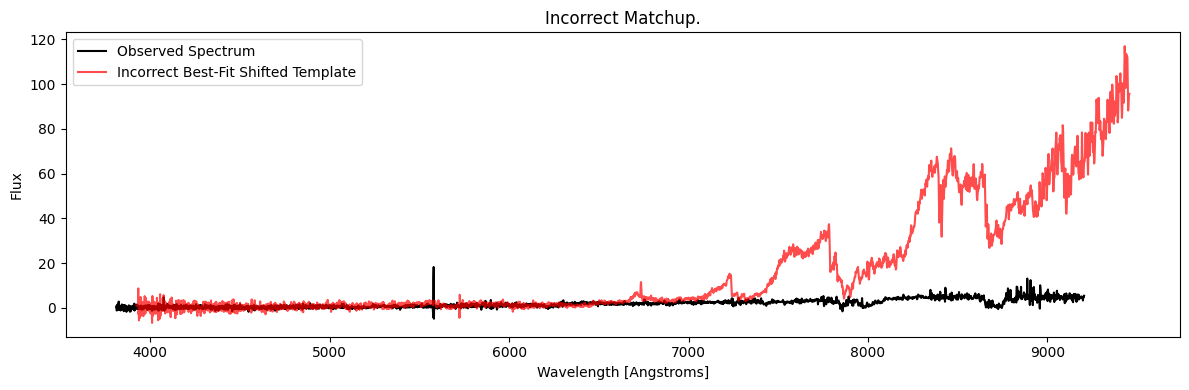
\includegraphics[width=1\linewidth]{image3.png}
    \caption{Incorrect Matchup}
    \label{fig:placeholder}
\end{figure}

\section{Conclusion}

Through a series of iterations, a working redshift estimation pipeline was developed that can operate on both synthetic and real galaxy spectra. Starting with simple peak detection, the approach gradually incorporated cross-correlation, normalization, and continuum subtraction to improve robustness. Along the way, failures revealed the importance of realistic templates and preprocessing. This process demonstrates how the ability to debug and refine an algorithm is just as essential as understanding the science behind it.

%----------------------------
% REFERENCES
%----------------------------

\bibliographystyle{plain} % or try: apalike, ieee, unsrt
\bibliography{references}

\end{document}
